\documentclass[border=6pt]{standalone}
\usepackage{tikz}
\usetikzlibrary{arrows.meta,positioning,calc,shapes.geometric,fit,backgrounds,patterns,matrix,decorations.pathreplacing}
\begin{document}
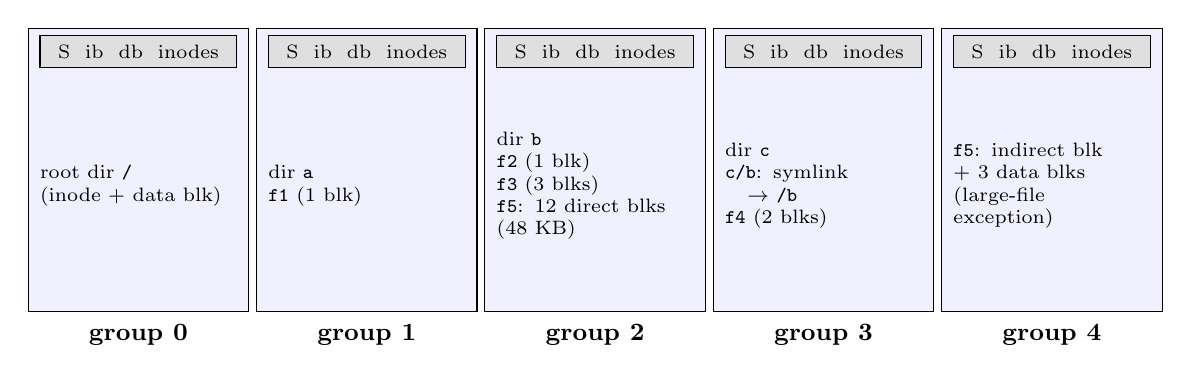
\begin{tikzpicture}[>=Stealth,font=\small]
\def\w{2.9}
\foreach \g/\txt in {0/{root dir \texttt{/}\\ (inode + data blk)},1/{dir \texttt{a}\\ \texttt{f1} (1 blk)},2/{dir \texttt{b}\\ \texttt{f2} (1 blk)\\ \texttt{f3} (3 blks)\\ \texttt{f5}: 12 direct blks\\ (48 KB)},3/{dir \texttt{c}\\ \texttt{c/b}: symlink\\ \quad$\to$ \texttt{/b}\\ \texttt{f4} (2 blks)},4/{\texttt{f5}: indirect blk\\ + 3 data blks\\ (large-file\\ exception)}}
{
 \draw[fill=blue!6] (\g*\w,0) rectangle (\g*\w+\w-0.1,3.6);
 \node[fill=gray!25,draw,minimum width=\w cm-0.4cm] at (\g*\w+\w/2-0.05,3.3) {\scriptsize S\ \ ib\ \ db\ \ inodes};
 \node[align=left,font=\scriptsize,text width=\w cm-0.4cm] at (\g*\w+\w/2-0.05,1.6) {\txt};
 \node[font=\small\bfseries] at (\g*\w+\w/2-0.05,-0.3) {group \g};
}
\end{tikzpicture}
\end{document}
